\section{MVC - \emph{Model View Controller.}}
\begin{frame}{Introducci\'on}
\begin{block}{}
	\begin{itemize}
		\item Patr\'on de diseño que separa al modelo de datos, la lógica de control de la aplicaci\'on y la interfaz de usuario en tres componentes distintos.
		\item Propone la implementaci\'on de 3 componentes caracterizados por:
			\begin{itemize}
				\item Tener muchas interfaces de usuario.
				\item Tener muchos controladores.
				\item Tener un solo modelo.
			\end{itemize}
	\end{itemize}
\end{block}
\end{frame}

\begin{frame}{Titulo}
	\begin{itemize}
		\item Modelo: Representaci\'on del modelo de dominio,  logica del negocio
		\item View: Interfaz de usuario e interacci\'on entre elementos de la interfaz.
		\item The controller: Intermediario entre modelo y vista, recibe los evntos ejecutados por el usuario y solicita al modelo los datos requeridos producto del evento.
		\end{itemize}
\end{frame}

\begin{frame}{Beneficios}
	\begin{itemize}
		\item Organizaci\'on.
		\item Desarrollo de aplicaci\'on r'apido.
		\item Reutilizaci\'on de c\'ondigo.
		\item Desarrollo de software paralelo.
		\item Permite representar la misma informaci\'on de distintas maneras.

	\end{itemize}
\end{frame}
%\begin{frame}{Tips - Ocultamiento de Informaci\'on - Ejemplo.}
  %\begin{figure}
    %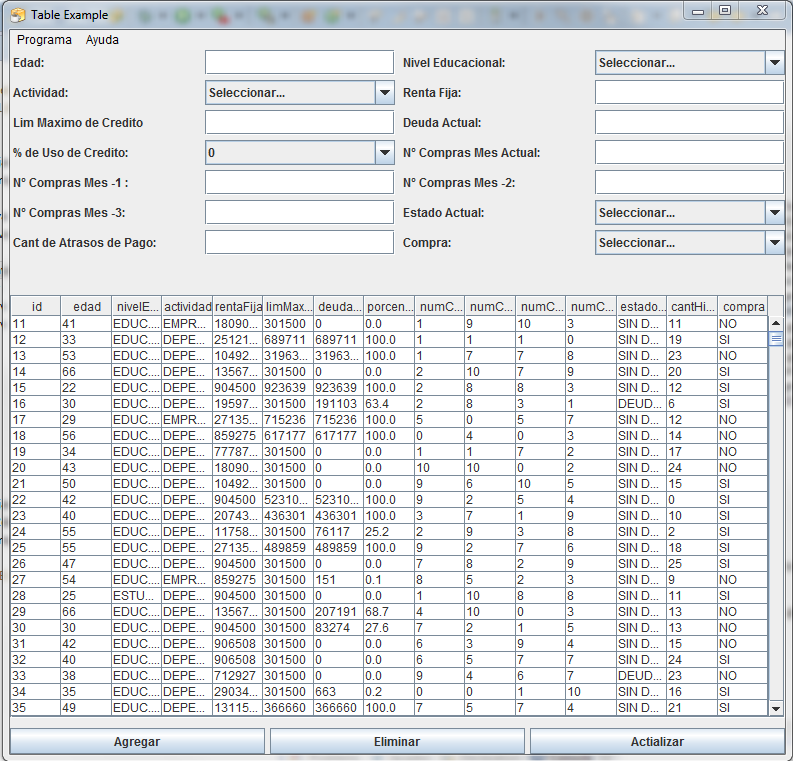
\includegraphics[scale=0.3]{figuras/DT.PNG}
  %\end{figure}
%\end{frame}

%\begin{frame}{Manejo de Excepciones - try, catch, finally}
%\begin{block}{Ejemplo.}
%\lstinputlisting[language=Java,caption={},numbers=none]{resources/excepciones/Finally.java}
%\end{block}
%\end{frame}
